\section{Introduction to Calling Conventions: Print}
In the previous section, we discussed throwing errors and how we can call an external (Rust) function from our generated assembly code. Note that the error case is interesting in the sense that it always terminated the program, so we didn't have to worry about coming back to our generated code.

\bigskip 

Suppose we want to introduce a \code{print} expression, which takes an expression and then prints the result out. Like the error handling, the \code{print} expression will call an external Rust function. However, unlike the error handling, we expect the \code{print} expression to come back to the generated assembly code \emph{after} calling the external function.

\bigskip 

Syntactically, \code{print} looks like 
\begin{verbatim}
    <expr> := ... | input | (print <expr>)\end{verbatim}

\subsection{Modifying \code{start.rs}}
Once again, as we need to define a function in Rust to handle printing so our generated assembly code can use it, we need to modify \code{start.rs} to include this information. Let's define the following function to handle printing: 
\begin{verbatim}
    #[no_mangle]
    #[export_name = "\01snek_print"]
    fn snek_print(val : i64) -> i64 {
        if val == 3 { println!("true"); }
        else if val == 1 { println!("false"); }
        else if val % 2 == 0 { println!("{}", val >> 1); }
        else {
            println!("Unknown value: {}", val);
        }
        return val;
    }\end{verbatim}
Note that 
\begin{itemize}
    \item \code{3} is our representation of \code{true} (\code{3} is \code{0b11} in binary.)
    \item \code{1} is our representation of \code{false} (\code{1} is \code{0b01} in binary.)
\end{itemize}

\subsection{Calling Convention Idea}
At a high level, when calling a function, we need to do the following: 
\begin{enumerate}
    \item ``Remember where'' we left off (i.e., recovering the stack).
    \item Pass in the appropriate arguments. 
    \item Call the \code{snek\_print} function.
\end{enumerate}
Regarding ``remember where'' we left off: remember that our compiler function has a parameter which represents the stack index. This stack index tells us how ``deep'' we are in the expressions that needed temporary storage/variables. So, whatever stack index we have, we need to set up the call so that it's above the stack index; after the call is done, we need to go back to where the stack index was originally.

\subsection{Implementing \code{print}}
Let's now attempt to implement \code{print} into our compiler.

\subsubsection{Attempt 1}
Our initial implementation of \code{print} might look like 
\begin{verbatim}
match e {
    ... 
    | Expr::Id(s) if s == "input" => "mov rax, rdi".to_string(),
    | Expr::Print(val) => {
        let offset = si * 8; 
        let v_is = compile_expr(val, si, env, l);
        format!("
            {v_is}
            sub rsp, {offset}
            mov rdi, rax 
            call snek_print
            add rdi, {offset}
        ")
    }
}\end{verbatim}
In terms of what's going on, what \verb|sub rsp, {offset}| is doing is moving \code{rsp}, the stack pointer, so that it's pointing \emph{above} where all the local variables and temporaries are.  
\begin{center}
    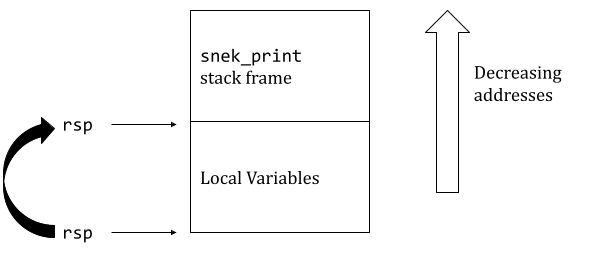
\includegraphics[scale=0.5]{assets/rsp_offset_subtract.png}
\end{center}
So, the stack frame for the \code{snek\_print} is where all the work for this function will happen. So, being its own function, it will rely on \code{rsp} being ``kind of'' like at bottom of its stack frame, since it gets its own local variable space whatnot. 

\begin{mdframed}
    (Exercise.) Consider the following code: 
    \begin{verbatim}
(block 
    (print 37)
    (print input)
)\end{verbatim}
    Using our implementation above, what would be printed if \code{input} was \code{true}? 

    \begin{mdframed}
        This would print \code{37} twice. To see why, let's consider the generated assembly.
        \begin{verbatim}
            mov rax, 74
            sub rsp, 16 
            mov rdi, rax 
            call snek_print 
            add rsp, 16 
            mov rax, rdi 
            ... \end{verbatim}
        The issue is in the third line, \code{mov rdi, rax}. We're overwriting \code{rdi}, which contains the result of \code{input}, with a different value! More specifically, we used \code{rdi} to pass in the argument for \code{print}, but this means we lose the result of \code{rdi} when we passed in the argument.
    \end{mdframed}
\end{mdframed}
So, we just need to remember to store data from registers somewhere else before we do the call. One thing we can do is store \code{rdi} somewhere on the stack before we make the function call. To do this, we can make use of \code{push} and \code{pop}. In fact, \code{rdi} is an example of a \textbf{caller-saved register}; that is, before we make a function call, we should save this register if we want to restore it afterwards. 

% https://stackoverflow.com/questions/9268586/what-are-callee-and-caller-saved-registers 

\subsubsection{Attempt 2}
With what we just mentioned in mind, we have 
\begin{verbatim}
    match e {
        ... 
        | Expr::Id(s) if s == "input" => "mov rax, rdi".to_string(),
        | Expr::Print(val) => {
            let offset = si * 8; 
            let v_is = compile_expr(val, si, env, l);
            format!("
                {v_is}
                sub rsp, {offset}
                push rdi            ; added this line 
                mov rdi, rax 
                call snek_print
                pop rdi             ; added this line 
                add rdi, {offset}
            ")
        }
    }\end{verbatim}
\textbf{Remark:} Remember that we want \code{rsp} to point to the spot where the pop is going to be, which is why we call \code{pop rdi} immediately after the \code{call} call. 

\bigskip 

Note that 
\begin{itemize}
    \item \code{push} pushes a value (register, immediate, etc.) to the stack. \code{push} will subtract 1 from \code{rsp}. 
    \item \code{pop} pops whatever is on top of the stack into a register. \code{pop} will add 1 to \code{rsp}. 
\end{itemize}
\begin{mdframed}[nobreak=true]
    (Example.) For example, 
    \begin{verbatim}
        push 17 
        push 23 
        pop rax 
        pop rcx \end{verbatim}
    will put \code{23} into \code{rax}, and \code{17} into \code{rcx}.
\end{mdframed}
So, in terms of what the generated assembly would do, it would 
\begin{itemize}
    \item Push \code{rsp} into the stack. 
    \item Then, move \code{rax} into \code{rsp}.
    \item Then, call the \code{snek\_print} function. 
    \item Then, put the most recently added value from stack (i.e, the old value of \code{rsp}) to the register \code{rsp}.
\end{itemize}
It just so happens that, in our example here, we only really care about \code{rdi}. But, if we have other registers that we care about (e.g., we use them a lot or need to save them between expressions), we need to save them. 

\subsection{Alignment Issues}
To summarize some of the things we've said about the x86\_64 calling convention\footnote{These are calling conventions specific to x86\_64, and is the reason why we had to do this when calling \code{snek\_print}. However, when we define our own functions in our own language, we can use whatever calling convention we want (including making one up) as long as it's consistent. }:
\begin{itemize}
    \item Arguments go into \code{rdi}, and then 6 other registers, and then the stack.
    \item \code{[rsp]} (i.e., the value stored at location \code{rsp}) should be the return pointer.
    \item 16-byte alignment constraint: $\code{rsp} \Mod{16} = 0$.
\end{itemize}
So, in our generated assembly, the third point may cause some problems with the stack pointer. One way we can resolve this is to check what $\code{stack\_offset} \Mod{16}$ is, or equivalently $\code{stack\_index} \Mod{2}$ is. For the latter, if we have an odd number, we can add 1 to the stack index so we have an even stack index.